\chapter{Modules}
\label{hoofdstuk:modules}
In dit hoofdstuk komen de voor dit thesisproject ontwikkelde modules aan bod. Zij proberen elk de collectie paarvoorstellen op een andere manier voor te stellen om een beter overzicht te cre\"eren of sneller individuele paren te beoordelen.\\

Modules kunnen ervoor kiezen het model dat ze toegewezen krijgen te manipuleren of niet. Indien wel, zullen alle modules die dit model delen steeds de veranderingen volgen.

\section{MatchTileView}
\emph{MatchTileView} is de meest uitgewerkte module en stelt 

Let uit wat de doorsnedes doen petra~\cite{Brown2010}

\begin{figure}[ht]
	\begin{center}
		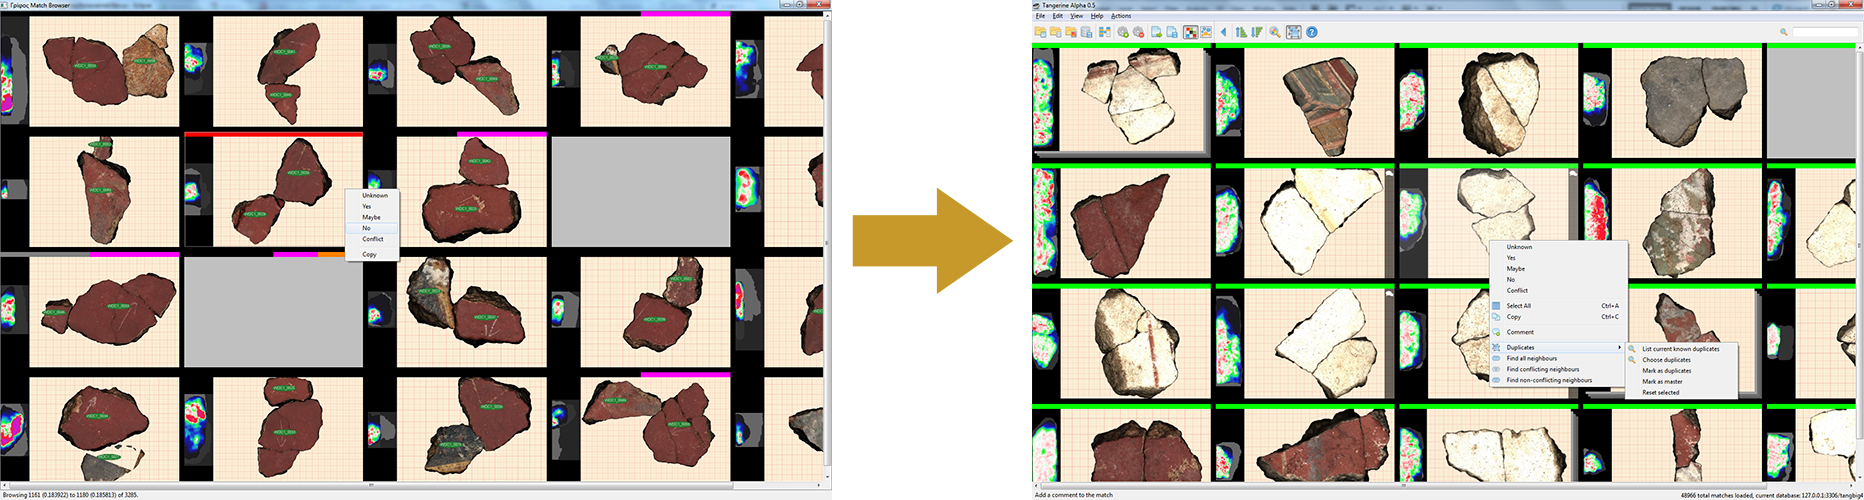
\includegraphics[width=1.0\columnwidth]{images/browsematches-to-tangerine-01.png}
		\caption{De manier van weergeven uit Browsematches werd gekopi\"eerd naar het nieuwe platform, met uitbreidingen}
		\label{fig:browsematchestotang}
	\end{center}
\end{figure}

De module gebruikt een paar visuele hints om aan te duiden dat er meer informatie beschikbaar is.
Het aanwezig zijn van commentaar 

Conflicten, verzamelingsreductie door conflicten (hoeveel percentage kan zo uitgeruled worden?) ---> space-filling curve

zoeken naar buren, niet conflicterende buren, duplicaten aanduiden, icoonbalken voor commentaren, DetailView, blabla

\subsection{Zoekfunctionaliteit}

\subsubsection{Buren}

Context is belangrijk

\subsubsection{DetailView}
\emph{DetailView} is geen normale module, het maakt geen gebruik van het parenmodel als databron. Het werkt eerder zoals de weergave in Griphos, waar de data-eenheid een geplaatst fragment is (zoals een puzzel).

Het belang van context

\section{Proof of concept: GraphView}
Pure grafische plugins kunnen vertrouwen op andere plugins voor data-selectie: Om de werkbaarheid van dit systeem uit te testen werd een voorbeeldmodule ontwikkeld die alle huidige paren op een graaf plaatst en hier een ontwarringsalgoritme op uitvoert. Deze voorstelling geeft een globaler beeld van de voortgang van de reconstructie zodat men een globaler beeld kan krijgen van de huidige selectie.

De \emph{GraphView} module vertouwt op een gedeeld model, aangezien het zelf geen zoekfunctionaliteit bevat. Dit betekent 